\documentclass{assignment}

\author{Артемий Сазонов}
\title{Домашняя работа по курсу <<Теория риска и стохастическая финансовая математика>>}
\date{\today}

\begin{document}
    \maketitle
    %\tableofcontents
    \setcounter{chapter}{7}
    %\part{Теория риска}
    %\setcounter{ProblemNum}{0}\chapter{}
    %\setcounter{ProblemNum}{0}\chapter{Модели индивидуального и коллективного риска, распределения убытков и их числа, классы Панджера, составные считающие распределения}
    \problem{}
        Проверить, что геометрическое распределение с $p_k = \P(X=k) = pq^k$, $k = 0, 1, \dots$ 
        обладает отсутствием памяти, т.е. 
        \begin{equation*}
            \P(X \geq k+l \vert X \geq k) = \P(X \geq l).
        \end{equation*}
    \solution{}
        \begin{multline*}
            \P(X \geq k+l \vert X \geq k) =\\= \frac{\P(X \geq k+l, X \geq k)}{\P(X \geq k)} = \frac{\P(X \geq k+l)}{\P(X \geq k)} = \\ =
            \frac{\sum _{n\geq k+l}pq^{n}}{\sum _{n\geq k}pq^{n}} = \frac{\sum _{n\geq k+l}q^{n}}{\sum _{n\geq k}q^{n}} = 
            \frac{\frac{q^{k+l}}{1-q}}{\frac{q^{k}}{1-q}} = q^l =\\= \frac{1-q}{1-q}q^l = \underbrace{(1-q)}_{=p} \frac{q^l}{1-q} = \sum_{n\geq l} pq^n = \P(X\geq l).
        \end{multline*}
    \problem{}
        Проверить, что производящая функция моментов случайной величины $S^{col} = \sum_{i=1}^{N} X_i$, где $N$ -- целочисленная случайная величина, не зависящая от последовательности н.о.р. случайных величин $(X_i)_{i \geq 1}$, записывается следующим образом:
        \begin{equation*}
            g_{S^{col}}(t) = \E \left[e^{tS^{col}}\right] = P_N(g_X(t)),
        \end{equation*}
        где $P_N(z) = \E \left[z^N\right]$ -- производящая функция $N$, а $g_X(t) = \E \left[e^{tX_i}\right]$ -- производящая функция моментов случайных величин $X_i$. Найти математическое ожидание и дисперсию величины $S^{col}$.
    \solution{}
        \begin{multline*}
            \E \left[e^{tS^{col}}\right] = \E \left[e^{t\sum_{i=1}^{N} X_i}\right] = \E \left[\left.\E\left[ e^{t\sum_{i=1}^{N} X_i}\right| N=n\right]_{n=N}\right] = \\ =
            \E \left[\E\left[ e^{t\sum_{i=1}^{n} X_i}\right]_{n=N}\right] = \E \left[\E\left[ e^{tX_i}\right]^n_{n=N}\right] = 
            \E \left[ \E[e^{tX_i}]^N\right] = P_N(g_X(t))
        \end{multline*}
        Из курса теории вероятностей знаем, что есть формула для моментов случайной величины, выраженных через производные производящей функции моментов:
        \begin{equation*}
            \E\left[(S^{col})^n\right] = \left.\frac{d^n \MGF_{S^{col}} (t)}{dt^n}\right|_{t=0+}
        \end{equation*}
        Итого имеем:
        \begin{align*}
            \E\left[S^{col}\right]     &= P_N'(g_X(0)) g_X'(0) =  P_N'(1) \E\left[X\right], \\ \\
            \E\left[(S^{col})^2\right] &= P_N''(g_X(0))\cdot (g_X'(0))^2 + P_N'(g_X(0))\cdot g_X''(0) =\\
                                       &= P_N''(1)\cdot (\E\left[X\right])^2 + P_N'(1)\var X, \\ \\
            \var S^{col}               &= P_N''(1)\cdot (\E\left[X\right])^2 + P_N'(1)\var X - \left(P_N'(1) \E\left[X\right]\right)^2 = \\ 
                                       &= \left(P_N''(1) - P_N'(1)^2\right)\E\left[X\right]^2 + P_N'(1)\var X.
        \end{align*}
    \problem{}
        Коэффициент изменчивости случайной величины $X$ равен $\cv X = \frac{\std X}{\E\left[X\right]}$. Пусть
        \begin{align*}
            S_1^{col} &= \sum_{i=1}^{N_1} Y_i, \\
            S_2^{col} &= \sum_{i=1}^{N_2} Z_i,
        \end{align*}
        где $N_1 \sim NB(10, 0.9)$, $N_2 \sim NB(1, 0.1)$, i.i.d. $Y_i \sim Exp (a)$, i.i.d. $Z_i \sim Par(x_0, 9/4)$. Найти коэффициенты изменчивости для $N_1$, $N_2$, $Y$, $Z$, $S_1$, $S_2$.
        Используемые обозначения:
        \begin{itemize}
            \item Отрицательное биномиальное распределение с параметрами $m$ и $p$:
                \begin{equation*}
                    N \sim NB(m, p) \iffdef \P(N = k) = C_{m+k-1}^{k}p^m(1-p)^k;
                \end{equation*}
            \item Показательное распределение с параметром $a$:
                \begin{equation*}
                    Y \sim Exp(a) \iffdef p_Y(x) = ae^{-ax}\1(x \geq 0);
                \end{equation*}
            \item Распределение Парето с параметрами $x_0$ и $d$:
                \begin{equation*}
                        Z \sim Par(x_0, d) \iffdef P(Z > x) = \left(\frac{x_0}{x}\right)^d\1(x > x_0).
                \end{equation*}
        \end{itemize}
    \solution{}
        \partsol{}
            Найдем коэффициент изменчивости для $N\sim NB(m, p)$.
            \begin{equation*}
                \left. \begin{aligned}
                    \E \left[N\right] &= \frac{pm}{1-p} & \\
                    \var N            &= \frac{pm}{(1-p)^2} 
                \end{aligned} \right\} \implies \cv N = \frac{\sqrt{\frac{pm}{(1-p)^2} }}{\frac{pm}{1-p}} = \frac{1}{\sqrt{pm}}.
            \end{equation*}
            В частных случаях:
            \begin{itemize}
                \item $(m, p) = (10, 0.9)\colon\quad \cv N_1 = \frac{1}{3}$,
                \item $(m, p) = (1, 0.1)\colon\quad\ \ \cv N_2 = 1$.
            \end{itemize}
        \partsol{}
            Найдем коэффициент изменчивости для $Y\sim Exp(a)$.
            \begin{equation*}
                \left. \begin{aligned}
                    \E \left[Y\right] &= \frac{1}{a} & \\
                    \var Y            &= \frac{1}{a^2} 
                \end{aligned} \right\} \implies \cv Y = \frac{\sqrt{\frac{1}{a^2}}}{\frac{1}{a}} \equiv 1.
            \end{equation*}
        \partsol{}
            $\cv S_1^{col}$ будем считать используя задачу 4. Условная плотность суммы:
            \begin{equation*}
                p_S(x|N) = \frac{a^N x^{N-1}}{\Gamma(N)}e^{-ax}\1(x\geq 0).
            \end{equation*}
            \begin{multline*}
                \E\left[S_1^{col}|N\right] = \int_{0}^{\infty} x\frac{a^N x^{N-1}}{\Gamma(N)}e^{-ax}dx = 
                \frac{1}{a\Gamma(N)} \int_{0}^{\infty} (ax)^{N}e^{-ax}d(ax) =\\= \frac{1}{a\Gamma(N)} \int_{0}^{\infty} y^{(N+1)-1}e^{-y}dy = \frac{\Gamma(N+1)}{a\Gamma(N)} = \frac{N}{a}
            \end{multline*}
            \begin{multline*}
                \E\left[(S_1^{col})^2|N\right] = \int_{0}^{\infty} x^2\frac{a^N x^{N-1}}{\Gamma(N)}e^{-ax}dx = \frac{1}{a\Gamma(N)} \int_{0}^{\infty} (ax)^{N+1}e^{-ax}dx =\\=
                \frac{1}{a^2\Gamma(N)} \int_{0}^{\infty} y^{(N+2)-1}e^{-y}dy = \frac{\Gamma(N+2)}{a^2\Gamma(N)} =\frac{N(N+1)}{a^2}
            \end{multline*}
            \begin{equation*}
                \var\left[S_1^{col}|N\right] = \frac{N(N+1)}{a^2} - \left(\frac{N}{a}\right)^2 = \frac{N}{a^2}
            \end{equation*}
            Итого,
            \begin{align*}
                \E\left[S_1^{col}\right] &= \E\left[\E\left[S_1^{col}|N\right]\right] = \E\left[\frac{N}{a}\right] = \frac{\frac{10\cdot 0.9}{1-0.9}}{a} = \frac{90}{a}, \\
                \var S_1^{col}           &= \E\left[\var\left[S_1^{col}|N\right]\right] = \frac{\frac{10\cdot 0.9}{1-0.9}}{a^2} = \frac{90}{a^2}, \\
                \cv S_1^{col}            &= \frac{\sqrt{10}}{30}.
            \end{align*}
        \partsol{}
            Тут посчитаем проще: $N = \sum_{k\in\mathbb{Z}}k\1(N=k)$, 
            \begin{align*}
                \E\left[S_2^{col}\right] &= \sum_{k\in \mathbb{N}\cup\{0\}}\left(C_{m+k-1}^{k}p^m(1-p)^k \sum_{i=1}^{k}\E\left[Z_i\right]\right) =\\&= \sum_{k\in \mathbb{N}\cup\{0\}}C_{m+k-1}^{k}p^m(1-p)^k k\E\left[Z\right] = \E\left[Z\right] \E\left[N_2\right] =\\&= \frac{9/4 \cdot x_0}{5/4} \cdot \frac{1}{0.9} = \frac{9 \cdot 10}{5\cdot 9}\cdot x_0 = 2x_0,\\
                \var S_2^{col}           &= \E\left[N_2\right]\var Z = \frac{1}{0.9} \frac{x_0^2} \cdot 9/4{(5/4)^2\cdot 1/4} = \frac{10\cdot 9}{9 \cdot (5/4)^2}x_0^2 = 6.4 x_0^2, \\
                \cv  S_2^{col}           &= \frac{\sqrt{6.4 x_0^2}}{2x_0} = \frac{\sqrt{6.4 x_0^2}}{2} = \sqrt{1.6} = \frac{4\sqrt{10}}{10}. 
            \end{align*}
    \problem{}
        Пусть $V_i$ имеет распределение $\Gamma(\alpha_i, \beta)$, $i=1,\dots, n$ с плотностью
        \begin{equation*}
            f_{V_i}(x) = \frac{\beta^{\alpha_i}x^{\alpha_i-1}}{\Gamma(\alpha_i)}e^{-\beta x}\1(x\geq 0).
        \end{equation*} 
        Величины $(V_i)_{i=1,\dots,n}$ независимы. Используя преобразование Лапласа показать, что $S^{ind} = \sum_{i=1}^{n} V_i$ имеет распределение $\Gamma(\sum_{i=1}^n \alpha_i, \beta)$.

    \solution{}
        Знаем, что у $X \sim \Gamma(\alpha, \beta)$
        \begin{equation*}
            \MGF_{X}(\lambda) = \left(1-\frac{\lambda}{\beta}\right)^{-\alpha}.
        \end{equation*}
        Итого имеем:
        \begin{multline*}
            \MGF_{S^{ind}}(\lambda) = \MGF_{\sum_{i=1}^{n} V_i}(\lambda) \overset{\text{в силу независимости}}{=\!=\!=\!=} \prod_{i=1}^n \MGF_{V_i}(\lambda) = \\ = \prod_{i=1}^n \left(1-\frac{\lambda}{\beta}\right)^{-\alpha_i} = \left(1-\frac{\lambda}{\beta}\right)^{-\sum_{i=1}^n \alpha_i}  = \MGF_{\Gamma(\sum_{i=1}^n \alpha_i, \beta)}(\lambda).
        \end{multline*}
            
    %\setcounter{ProblemNum}{0}\chapter{Суммарный размер ущерба. Динамические модели. Модель Крамера - Лундберга и вероятность разорения}
    \problem{}
        Показать, что логарифмически нормальное распределение масштабно инвариантно, но не обладает масштабным параметром.
    \solution{}
        \begin{definition}[Масштабно инвариантное семейство]
            Семейство распределений называется масштабно инвариантным, если вместе с распределением случайной величины $X$ распределение $Y=cX \quad \forall c \in \mathbb{R^+}$ также принадлежит этому семейству.  
        \end{definition}
        $X\sim LN(a, \sigma^2)$, т.е. $\exists Y \sim N(a, \sigma^2)\colon \ X = \exp \left\{ Y \right\}$.
        Посмотрим, какое распределение у $cX$:
        \begin{equation*}
            cX = c\exp\left\{Y\right\} = \exp\left\{Y + \log c\right\},
        \end{equation*}
        т.е. $cX \sim LN(a+\log c, \sigma^2)$.

    \problem{}
        Доказать, что пуассоновское распределение $Pois(\lambda)$ получается из отрицательно биномиального распределения $NB(\alpha, \beta)$, если положить $\lambda = \alpha(1 - \beta)$ и $ \beta \to 1$.
    \solution{}
        \begin{definition}
            [Отрицательное биномиальное распределение $NB(m, p)$]
                \begin{equation*}
                        \P(X = k) =\tbinom{m+k-1}{k} p^m(1-p)^k \iff \MGF_X(t) = \left(\frac{1-p}{1-pe^t}\right)^m.
                \end{equation*}
        \end{definition}
        Пусть $X\sim NB(\alpha, \beta), \alpha\beta=:\lambda$. Найдем предельную $MGF$ при $\beta\to 0$:
        \begin{multline*}
            \lim_{\beta\to 0}\MGF_X(t) = \lim_{\beta\to 0} \left(\frac{1-\beta}{1-\beta e^t}\right)^\alpha = \\ =
            \lim_{s\to 0}  \left(\frac{1-s}{1-se^t}\right)^{\lambda / s} = 
            \lim_{s\to 0}  \left(\frac{1-se^t}{1-s}\right)^{-\lambda / s} \overset{\text{из 2 зам.пр.}}{=\!=\!=\!=\!=\!=} e^{\lambda \left( e^{t}-1 \right) } = \MGF_{Pois(\lambda)}(t).
        \end{multline*} 
        По теореме о характеризации получаем, что предельное распределение пуассоновское ($\MGF \leftrightarrow \law$).

    \problem{}
        Все ли распределения класса $(a, b, 0)$ являются безгранично делимыми?
    \solution{}
        \begin{definition}
            Считающее распределение принадлежит классу $(a, b, 0)$, если 
            \begin{equation*}
                p_k = p_{k-1}\left( a+\frac{b}{k} \right).
            \end{equation*}
            При этом $p_0 = 1-\sum_{k = 1}^\infty p_k$
        \end{definition}
        Знаем, что только $Pois, B, NB, Geom$\footnote{$Geom$ частный случай $NB$} принадлежат этому классу.
        \begin{definition}
            Случайная  величина $Y$ (ее распределение) называется бесконечно делимой (-ым), если для любого $n \in \mathbb{N}$ она может быть представлена в виде $Y = \sum_{i=1}^n X^{(n)}_i$, где  $(X_i^{(n)})_{i=1\dots n}$ -- независимые одинаково распределённые случайные величины.
        \end{definition}
        \begin{itemize}
            \item $Pois(\lambda)$: берем $n$ н.о.р. $Pois(\lambda/n)$ случайных величин;
            \item $B(m, p)$ \begin{equation*}
                \MGF_{B(m, p)} = \left(1-p + pe^t\right)^m = \left(\left(\sqrt[n]{1-p + pe^t}\right)^m\right)^n;
            \end{equation*}
            \item $NB(m, p)$ \begin{equation*}
                \MGF_{NB(m, p)} = \left(\frac{1-p}{1-pe^t}\right)^m = \left(\left(\sqrt[n]{\frac{1-p}{1-pe^t}}\right)^m\right)^n.
            \end{equation*}
        \end{itemize}
    \problem{}
        Выписать явный вид $(p^T_k)_{k\geq 1}$ для урезанных в нуле распределения из класса $(a, b, 0)$.
    \solution{}
        $p^T_k = \frac{p_k}{(1 -p_0)}$. Далее $k\geq 1$.
        \begin{itemize}
            \item $TB(n, p)$
            \begin{equation*}
                p_k^T = \binom{n}{k} \frac{p^k(1-p)^{n-k}}{1 - (1-p)^n};
            \end{equation*}
            \item $TPois(\lambda)$
            \begin{equation*}
                p^T_k = \frac{1}{k!} \frac{\lambda ^ k }{e^\lambda - 1};
            \end{equation*}
            \item $TNB(\alpha, \beta)$
            \begin{equation*}
                p_k^T = \tbinom{k + \alpha - 1}{k}\frac{\beta^{k}}{(1+\beta)^{\alpha+k} - (1+\beta)^k};
            \end{equation*}
            \item $TGeom(\beta)$
            \begin{equation*}
                p_k^T = \frac{\beta^{k - 1}}{(1 + \beta)^k}.
            \end{equation*}
        \end{itemize}
    %\setcounter{ProblemNum}{0}\chapter{Меры опасности. Порядки на случайных величинах.}
    \problem{}
        Пусть $f_X(x) = \exp\{ - |x/\theta | \}/2\theta$ для $-\infty < x < \infty$, $\theta>0$. Найти распределение $Y=e^X$.

        \solution{}
            $\P(Y < 0) = 0$. Пусть $x>0$. Тогда 
            \begin{equation*}
                \P (Y \leq x) =  \P ( X \leq \ln x) \quad \implies \quad f_Y(x) = f_X(\ln x)/x \1(x>0). 
            \end{equation*}
            Значит $f_Y(x) = \exp \{-|\ln x /\theta |  \}/( 2\theta x) \cdot \1(x>0)$, где  $\1(x \in A)$ - индикаторная функция множества $A$, а функция распределения имеет следующий вид:
            \begin{equation*}
                F_X(x) = \frac{x^{1/\theta}}{2}  \1(0<x<1) + (1 - \frac{x^{-1/\theta}}{2}) \1(x\geq 1).
            \end{equation*}
    
    \problem{}
        Будет ли свертка составных пуассоновских распределений также составным пуассоновским распределением?
        \solution{}
            Пусть $\widetilde N_1$ и $\widetilde N_2$ - независимые составные пуассоновские распределения. Тогда их производящие функции имеют следующий вид: $P_{\widetilde N_i}(z) = \exp \{ \lambda_i (P_i(z) -1 ) \}, \quad i=1,2 $. Тогда
            \begin{equation*}
                P_{\widetilde N_1 + \widetilde N_2}(z) = P_{\widetilde N_1}(z) \cdot P_{\widetilde N_2}(z) = \exp \{\lambda_1 (P_1 (z) -1) + \lambda_2 (P_2(z) - 1) \}.
            \end{equation*}
            Чтобы получившееся распределение было составным пуассоновским необходимо и достаточно чтобы 
            \begin{equation*}
                \lambda_1 (P_1 (z) -1) + \lambda_2 (P_2(z) - 1) = \lambda ( P(z) - 1),
            \end{equation*}
            для некоторой MGF $P(z)$ и некоторого $\lambda>0$. Пусть $P_i(z) = \sum_{k=0}^\infty p_k^i z^k$, $P(z) = \sum_{k=0}^\infty p_k z^k$. Тогда
            \begin{equation} \label{system}
                \left\{\begin{aligned}
                    &\lambda_1p_k^1 + \lambda_2p_k^2 - \lambda p_k = 0,\qquad k=1,2,\dots \\
                    &\lambda_1p_0^1 + \lambda_2 p_0^2 - \lambda p_0 = \lambda_1 + \lambda_2 - \lambda\\
                    &p_k \geq 0, \quad k = 0,1,2 \dots\\
                    &\sum _{k=0}^\infty p_k = 1\\
                    &\lambda > 0
                \end{aligned}\right.
            \end{equation}
            откуда находим 
            \begin{equation*}
                \left\{\begin{aligned}
                    &p_k = \frac{\lambda_1p_k^1 + \lambda_2p_k^2}{\lambda}, \quad k = 1, 2, \dots\\
                    &\lambda = \frac{\lambda_1(1 - p_0^1) + \lambda_2 ( 1 - p_0^2)}{1 - p_0}.
                \end{aligned}\right.
            \end{equation*}
            Откуда видно, что $\lambda > 0$, если $p_0^1 < 1$ или $p_0^2 < 1$. В этом случае и все $p_k \geq 0$. Осталось проверить условие, что $\sum _{k=0}^\infty p_k = 1$. 
            \begin{equation*}
                \sum _{k=0}^\infty p_k = p_0 + \sum _{k=1}^\infty p_k = p_0 + \frac1\lambda \sum _{k=1}^\infty \left( \lambda_1 p_k^1 + \lambda_2 p_k^2 \right) = p_0 + \frac{\lambda_1 (1 - p_0^1) + \lambda_2 ( 1 - p_0^2)}{\frac{\lambda_1(1 - p_0^1) + \lambda_2 ( 1 - p_0^2)}{1 - p_0}} = 1.
            \end{equation*}
            Итак, зафиксировав $p_0 < 1$ мы однозначно найдем производящую функцию $P(z)$ и $\lambda>0$ из системы \eqref{system}, если $p_0^1<1$ и  $p_0^2 < 1$. Если же $p_0^1=p_0^2 = 1$, то подойдет $P(z) = 1$ и произвольное $\lambda > 0$. В любом случае, получаемя, что свертка составных пуассоновских распределений есть составное пуассоновское распределение.

    \problem{}
        Проверить, что отрицательное биномиальное распределение - это пуассоновско-логарифмическое распределение. 
        \solution{}
            Логарифмическое распределение определяется следующим образом
            \begin{equation*}
                p_k = \frac{\frac{\beta^k}{(1+\beta)^k}}{k\ln(1 + \beta)}, \quad k=1,2,\ldots.
            \end{equation*}
            Найдем производящую функцию логарифмического распределения. Пусть $z\leq 1$. Тогда
            \begin{align*}
                &\sum\limits_{k=1}^\infty p_k = \sum\limits_{k=1}^\infty \frac{\frac{\beta^k}{(1+\beta)^k}}{k\ln(1 + \beta)}z^k = \frac{\beta}{(1+\beta)\ln(1 + \beta)} \int\limits_0^z 
                \sum\limits_{k=0}^\infty \left( \frac{\xi \beta}{1 + \beta} \right)^k d\xi= \\
                &= \frac{\beta}{(1+\beta)\ln(1 + \beta)} \int\limits_0^z \frac1{1 - \frac{\xi \beta}{1 + \beta}} d\xi
                = -\frac{\ln(1 - \frac{z \beta}{1 + \beta} )}{\ln(1+\beta)}.
            \end{align*}
            Тогда производящая функция пуассоновско-логарифмического распределения выглядит следующим образом:
            \begin{equation*}
                \exp\left\{ \lambda\left(-\frac{\ln(1 - \frac{z \beta}{1 + \beta} )}{\ln(1+\beta)} - 1\right) \right\} =  \exp\left\{ \lambda\left(-\frac{\ln(1 + \beta - z \beta )}{\ln(1+\beta)}\right) \right\} = \left(1 + \beta - z \beta \right)^{-\frac{\lambda}{\ln(1 + \beta)}}.
            \end{equation*}
            Производящая функция отрицательного биномиального распределения $NB(a,b)$ имеет следующий вид:
            \begin{equation*}
                (1+b+bz)^{-a}.
            \end{equation*}
            Положив $\beta = b, \lambda = a\ln(1+b)$ получаем, что отрицательное биномиальное распределение является пуассоновско-логарифмическим.
    
    \problem{}
        Показать, что для составного пуассоновского распределения 
        \begin{equation*}
            g_n = \frac{\lambda}{n}\sum\limits_{j=1}^n jf_jg_{n-j}.
        \end{equation*}
        \solution{}
            Пуассоновское распределение $Pois(\lambda)$ принадлежит классу $(a, b, 0)$ с $a=0, b=\lambda, p_0 = e^{-\lambda}$. Пусть вторичное распределение задано $\{f_k \}_{k=0}^\infty$. Тогда по теореме Панджера имеем
            \begin{equation*}
                g_n = \frac1{1 - af_0} \sum\limits_{j=1}^n ( a + \frac{bj}n)f_j g_{n-j} = \frac{\lambda}{n} \sum\limits_{j=1}^n jf_j g_{n-j}.
            \end{equation*}
    
    \problem{}
    Если первичное распределение принадлежит классу $(a,b,1)$, то справедливо соотношение:
    $$g_n =\frac{[p_1 - (a + b)p_0]f_n +\sum^n_{j=1}\left(a + \frac{bj}{n}\right)f_j g_{n-j}}{1 - af_0}.$$
        
        \solution{}
            Рассуждения аналогичные доказательству теоремы Панджера. А именно: перепишем рекурентное соотношение в виде 
            \begin{equation*}
                kp_k = a(k-1)p_{k-1} + (a+b)p_{k-1} ,\quad k=2,3,\ldots .
            \end{equation*}
            Умножим обе части это равенства на $[P_2(z)]^{k-1}P^\prime_2(z)$ и просуммируем по $k$ начная с $k=2$:
            \begin{equation} \label{eq5_1}
            \sum\limits_{k=2}^\infty kp_k[P_2(z)]^{k-1}P^\prime_2(z) = a \sum\limits_{k=2}^\infty (k-1)p_{k-1}[P_2(z)]^{k-1}P^\prime_2(z) + (a+b)\sum\limits_{k=2}^\infty p_{k-1}[P_2(z)]^{k-1}P^\prime_2(z).
            \end{equation}
            Учитывая, что $P(z)=P_1(P_2(z)) = \sum\limits_{k=0}^\infty p_k[P_2(z)]^k$, получаем, что \ref{eq5_1} переписывается в виде:
            \begin{equation*}
                P^\prime(z) - p_1P^\prime_2(z) = aP_2(z)P^\prime(z) + (a+b)\left[P(z)P^\prime_2(z) - p_0P^\prime_2(z) \right].
            \end{equation*}
            Раскладывая левую и правую части в ряд и приравнивая коэффициенты при $z^{n-1}$ получаем:
            \begin{equation*}
                ng_n - np_1f_n = a \sum_{j=0}^n(n-j)f_jg_{n-j} + (a+b)\left[ \sum_{j=0}^njf_jg_{n-j} - np_0f_n\right].
            \end{equation*}
            Перенося в левую часть все слагаемы связаные с $g_n$ и группируя остальные получаем :
            \begin{equation*}
                g_n(n -anf_0) = nf_n[p_1 - (a+b)p_0 ] +  \sum_{j=1}^n(an + bj)f_jg_{n-j}.
            \end{equation*}
            Разделив обе части на $(n -anf_0)$ окончательно получаем:
            \begin{equation*}
                g_n =\frac{[p_1 - (a + b)p_0]f_n +\sum^n_{j=1}\left(a + \frac{bj}{n}\right)f_j g_{n-j}}{1 - af_0}.
            \end{equation*}
    %\setcounter{ProblemNum}{0}\chapter{Выпуклый порядок. Свойства инвариантности стоп-лосса. Сравнение биномиальной, пуассоновской и отрицательной биномиальной моделей.}
    \problem{}
        Пусть $<_b$ - полный порядок всех рисков для лица $b$ из некоторого множества $B$ лиц, принимающих решения. Определим бинарное отношение $<_a$ на множестве рисков следующим образом: $X<_a Y$ тогда и только тогда, когда $X<_bY$ для всех $b \in B$. Доказать, что $<_a$ - частичный порядок, (отражающий предпочтения всех лиц из мн-ва $B$).
        \solution{}
            Необходимо проверить свойства рефлексивности, транзитивности и антисимметричности. 
            \begin{itemize}
                \item[\textbf{Рефлексивность}] $X<X$. Возьмем произвольное $b \in B$. $X<_b X$ - поскольку $<_b$ - рефлексивно. В силу произвольности $b \in B$ получаем, что $X<_a X$.
                \item[\textbf{Транзитивность}] $X<Y,\; Y<Z \Rightarrow X<Z$.
                Пусть $X<_aY,\; Y<_a Z$. Значит $X<_b Y \; \forall b \in B$ и $Y<_b Z \; \forall b \in B$. Возьмем произвольное $b \in B$. Тогда, поскольку $<_b$ - полный порядок на множестве рисков для лица $b$, то $X<_b Z$ по транзитивности для порядка $<_b$. В силу произвольности $b \in B$ получаем, что $X<_a Z$.
                \item[\textbf{Антисимм-ть}] $X<Y, \; Y<X \; \Rightarrow X=Y$. Пусть $X<_aY$ и $Y<_aX$. Т.е. $X<_bY$ и $Y<_bX$ $\forall b \in B$. Возьмем произвольное $b \in B$. Из $X<_b Y$ и $Y<_b X$ следует, что $X=Y$ из антисимметричности $<_b$. В силу произвольности $b \in B$ получаем, что из $X<_aY$ и $Y<_aX$ следует, что $X=Y$.
                
            \end{itemize}
            Итак, мы доказали, что отношение $<_a$ обладает свойствами транзитивности, рефлексивности и антисимметричности. Значит отношение $<_a$ является частичным порядком на множестве всех рисков, который учитывет предпочтения всех лиц $b$ из множества $B$.
    
    \problem{}
        Предположим, что $X_1 <_{st} X_2$. Можно ли (на том же самом вероятностном пространстве) найти такую случайную величину $X^\prime_2$, чтобы $X_1 <_1 X^\prime_2$ и $X_2 \stackrel{d}{=} X^\prime_2$ ?
        \solution{}
            Определим вероятностное пространство следующим образом: $\Omega=\{0,1\},\; \mathcal{F} = 2^\Omega, \mathbb P(\{0\}) = \frac34, \mathbb P(\{1\}) = \frac14, \mathbb P(\Omega) = 1, \mathbb P(\varnothing) = 0$. Определим случайные величины как $X_2 = \textbf{1}_{\{0\}}(\omega), \; X_1 = \textbf{1}_{\{1\}}(\omega)$, где $\textbf{1}_{\{i\}}(\omega)$ - индикатор точки $i$. Легко видеть, что $X_1 <_{st} X_2$. Однако, не существует $X^\prime_2 \stackrel{d}{=} X_2$, т.ч. $X_1 <_1 X^\prime_2 $. Действительно, пусть существует. Тогда $X^\prime_2(1) \geq 1 = X_1(1)$. Поскольку $\mathbb P(X^\prime_2 = 0) = \mathbb P (X_2 = 0) =\frac14$ то $X^\prime_2(1) = 0$, так как $\mathbb P(A) = \frac{1}{4} \; \Leftrightarrow \; A=\{1\} $. Противоречие.
            
    \problem{}
        Доказать свойство $3^\circ$ непосредственно, пользуясь определением свертки. Будут ли выполнены свойства $1^\circ,2^\circ,4^\circ$ для стохастического порядка?
        \solution{}
            Свойство $3^\circ$: $F_1 \prec F_2, \; G: \; F_k*G \in B_{\prec},\; k=1,2 \; \Rightarrow \; F_1*G \prec F_2*G $.
                
            Пусть $F_1 <_{st} F_2$. Тогда $F_1(t) \geq F_2(t), \; \forall t  $. Тогда получаем, что 
            \begin{equation*}
                \int_{-\infty}^{\infty} \textbf{1}(x+y\leq t) dF_1(x) \geq \int_{-\infty}^{\infty} \textbf{1}(x+y\leq t) dF_2(x) , \; \forall y \in \mathbb R,
            \end{equation*}
            поскольку вариация функции $F_1(t)$ с учетом знака на луче $(-\infty, z]$ больше или равна вариации функции $F_2(t)$ на том же луче $\forall z \in \mathbb R$.
            Поскольку $G(t)$ - монотонно неубывает на всей прямой, то интеграл римана-стилтьесса сохраняет неравенства, т.е. 
            \begin{equation*}
                \int_{-\infty}^{\infty}\int_{-\infty}^{\infty} \textbf{1}(x+y\leq t) dF_1(x)dG(y) \geq \int_{-\infty}^{\infty}\int_{-\infty}^{\infty} \textbf{1}(x+y\leq t) dF_2(x)dG(y) , \; \forall y \in \mathbb R,
            \end{equation*}
            что равносильно 
            \begin{equation*}
                G*F_1 <_{st} G*F_2.
            \end{equation*}
    
    \problem{}
        Сохраняется ли стохастический порядок при взятии составных распределений?
        \solution{}
        Пусть $\{X_k\}_{k=1}^\infty$ - н.о.р., $N$ - неотрицательная, целочисленная случайная величина не зависящая от $\{X_k\}_{k=1}^\infty$, $p_k = \mathbb P(N=k)$. $S_n = \sum_{k=1}^n ,\; S_0 = 0$. Тогда 
        \begin{equation*}
            P(S_N\leq x) = \sum_{k=0}^\infty p_k\mathbb P(S_k \leq x) = \sum_{k=0}^\infty p_kF^{*k}(x).
        \end{equation*}
        Из задачи $2$ и замечания к задаче 2 следует, что если $F_1 <_{st}F_2$, то $F_1^{*k} <_{st} F_2^{*k}$. Действительно, для $k=1$ - это верно. Пусть верно для $k=n-1$, докажем для $k=n$. 
        \begin{equation*}
           F_1^{*(n-1)}<_{st} F_2^{*(n-1)} \; \Longrightarrow \; F_1^{*(n-1)}*F_2 <_{st} F_2^{*n}.
        \end{equation*}
        \begin{equation*}
            F_1<_{st} F_2 \; \Longrightarrow \; F_1^{*n} <_{st} F_1^{*(n-1)}*F_2
        \end{equation*}
        Пользуясь транзитивностью стохастического порядка получаем требуемое утверждение.
        
        Из определения стохастического порядка видно, что если $\sum_{k=0}^n p^n_k = 1,\; p^n_k\geqslant0$ и $F_{1,k}k <_{st} F_{2,k} \; \forall k$, то $\sum_{k=0}^np^n_kF_{1,k} <_{st} \sum_{k=0}^np^n_kF_{2,k} $, или, что тоже самое (по определению стохастического порядка) 
        \begin{equation}
            \sum_{k=0}^np^n_kF_{1,k}(t) \geq \sum_{k=0}^np^n_kF_{2,k}(t),\; \forall t\in \mathbb R.
        \end{equation}
        
        Переходя к пределу по $n$ в последнем неравенстве, получаем 
        \begin{equation*}
            \sum_{k=0}^\infty p_kF_{1,k}(t) \geq \sum_{k=0}^\infty p_kF_{2,k}(t),\; \forall t\in \mathbb R,
        \end{equation*}
        или, равносильно
        \begin{equation*}
            \sum_{k=0}^\infty p_kF_{1,k} <_{st} \sum_{k=0}^\infty p_kF_{2,k}.
        \end{equation*}
        Применяя все написаное выше непосредственно к нашей задаче, получаем: если $F_1 <_{st} F_2$, то
        \begin{equation*}
            \sum_{k=0}^\infty p_kF_1^{*k} <_{st} \sum_{k=0}^\infty p_kF_2^{*k}.
        \end{equation*}
        Итак, получаем следующее утверждение: пусть $\{X_k^i\}_{k=1}^\infty$ - н.о.р. с функцией распределения $F_i(x)$, $i=1,2$, $N$ - неотрицательная целочисленная с.в. . Пусть также $F_1 <_{st}F_2$. Определим $S^i_n=\sum_{k=1}^n ,\; S_0^i = 0$, $G_i(x) = \mathbb P(S_N \leq x) ,\; i=1,2 $. Тогда $G_1 <_{st} G_2$, т.е. взятие составного распределения сохраняет стохастический порядок. 
        
    \problem{}
        Если $\mathbb EX = m$, то $m<_{sl} X$.
        \solution{}
            Покажем, что $\mathbb E \max(d,m) \leq \mathbb E \max(d, X)$, что эквивалентно $m<_{sl}X$. Пусть $d>m$. Тогда $\max(d,m) = m$. Тогда $d\leq \max(d, X)$ и, следовательно $\mathbb Ed \leq \mathbb E\max(d,X)$. Пусть $m\geq d$. Тогда, поскольку $X\leq \max(d,X)$ и $\max(m,d) = m$,то $ m=\mathbb EX\leq \mathbb E \max(X,d)$. Итак, получили что $\forall d \in \mathbb R \;\;\; \mathbb E \max(d,m) \leq \mathbb E \max(d,X)$, т.е. $m<_{sl}X$.
            

    %\setcounter{ProblemNum}{0}\chapter{Тарифный принцип, нагрузка в явном и неявном виде. Порядок отношения правдоподобия и экспоненциальный порядок.}
\problem{}
Пусть число наступления событий $N$ имеет распределение Пуассона с параметром $\lambda$. События классифицируются на $m$ групп, причем каждое из них, независимо от остальных, принадлежит $i$-й группе с вероятностью $p_i$. Тогда случайные величины $N_i$, $i =\overline{1,m}$, независимые пуассоновские с параметрами $p_i\lambda$. ($N_i$ - число событий в группе $i$.)

\solution{}
    Пусть $\eta_k$ -- номер класса события $k$. Тогда
    \begin{equation}
        \P(\eta_k = i) = p_i.
    \end{equation}
    Из условия задачи имеем
    \begin{equation}
        N_i = \sum_{k:\ \eta_k = i} 1 = \sum_k \1(\eta_k = i).
    \end{equation}
    Найдем искомое распределение:
    \begin{multline}
        \P(N_i = n) =
        \sum_{k=0}^\infty \P\left(N=k, \sum_{n=1}^k\1(\eta_k = i) = n\right) =\\=
        \sum_{k=n}^\infty \P\left(N=k, \sum_{n=1}^k\1(\eta_k = i) = n\right) =\\=
        \sum_{k=n}^\infty \P\left(N=k\right) \P\left(\sum_{n=1}^k\1(\eta_k = i) = n\right) =\\=
        \sum_{k=n}^\infty \frac{\lambda^k}{k!}e^{-\lambda} \binom{k}{n}p_i^n(1-p_i)^{k-n} =\\=
        \sum_{k=n}^\infty e^{-\lambda} \frac{\lambda^k}{k!}\frac{k!}{n!(k-n)!} p_i^n(1-p_i)^{k-n} =\\=
        \sum_{k=n}^\infty e^{-\lambda} \frac{\lambda^k}{n!(k-n)!} p_i^n(1-p_i)^{k-n} =\\=
        \frac{p_i^ne^{\lambda}\lambda^n}{n!}\sum_{k=0}^\infty\frac{(\lambda(1-p_i))^{k}}{k!}  =
        \frac{(\lambda p_i)^n}{n!}e^{-\lambda p_i}.
    \end{multline}
    Получили искомое распределение. Остается проверить независимость. Это свойство очевидно следует из независимости $\eta_k$.

\problem{}
Проверить, что биномиальные распределения с параметрами $n$ и $p$ растут стохастически по $p$ при фиксированном $n$ и стохастически растут по $n$ при фиксированном $p$.

\solution{}
    1. Фиксируем $n$. Пусть $p_1 < p_2$. Тогда хотим
        \begin{equation}
            \P(X_1 = k) = \binom{n}{k}p_1^k(1-p_1)^{n-k} \geq \binom{n}{k}p_2^k(1-p_2)^{n-k} = P(X_2 = k).
        \end{equation}
        На биномиальный коэффициент можно не обращать внимания, так как он не зависит от $p$. Тогда нужно проверить неравенство
        \begin{equation}
            p_1^k(1-p_1)^{n-k} \geq p_2^k(1-p_2)^{n-k}.
        \end{equation}
        Обозначим $a = p_2/p_1 > 1, p_1 = p$. Имеем:
        \begin{equation}\label{to1}
             \underbrace{a^k}_{<1} \left(\frac{1-ap}{1-p}\right)^{n-k} <...?
        \end{equation}
        \begin{equation}
            \frac{1-ap}{1-p}\ \ ?\ \ 1
        \end{equation}
        \begin{equation}
            1-ap\ \ ?\ \ 1-p
        \end{equation}

        Отсюда следует, что $?$ это $<$. 
        Таким образом, в \eqref{to1} можно поставить $1$ вместо многоточия, и имеем стохастическую монотонность.

    2. Фиксируем $p$. Пусть $n_1 < n_2$. Тогда хотим
        \begin{equation}
            \P(X_1 = k) = \binom{n_1}{k}p^k(1-p)^{n_1-k} \geq \binom{n_2}{k}p^k(1-p)^{n_2-k} = P(X_2 = k).
        \end{equation}
        Хотим \begin{equation}
            \frac{n_1!}{(n_1 - k)!}(1-p)^{n_1} \geq \frac{n_2!}{(n_2 - k)!}(1-p)^{n_2}
        \end{equation}
        Хотим \begin{equation}
            \frac{n_1!}{n_2!}\frac{(n_2 - k)!}{(n_1 - k)!}(1-p)^{n_1-n_2} \geq 1
        \end{equation}
        Имеем
        \begin{equation}
            \frac{n_1!}{n_2!}\frac{(n_2 - k)!}{(n_1 - k)!}(1-p)^{n_1-n_2} \geq \frac{n_1!}{n_2!}\frac{(n_2 - n_1)!}{1}(1-p)^{n_1-n_2} > 1
        \end{equation}

\problem{}
Верно ли, что $D Y \geq D X$, если $X <_v Y$?

\solution{}
    Пусть $X <_v Y$. По определению это означает, что $\exists Z\colon \E\left[Z|X\right] \overset{\text{a.s.}}{\geq} 0$ и $X+Z \overset{\text{law}}{=} Y$.
    Более того, знаем, что $X<_vY \iff X<_{sl}Y, X<_{st}Y$. А отсюда следует необходимость данного стохастического порядка.
    Рассмотрим\begin{enumerate}
        \item $X \sim U[1, 3]$, $\var X = 1/3$;
        \item $Y\sim U[3, 4]$, $\var Y = 1/12$.
    \end{enumerate}
    Есть стохастический и стоп-лосс, а значит, выполнено $X<_vY$. Но $\var X > \var Y$, что противоречит условию.

\problem{}
Пусть риск $X$ равномерно распределен на $[0, 2]$, а $Y$ имеет показательное распределение с параметром 1, тогда $X <_{sl} Y$ .

\solution{}
    Пусть $0 < d < 2$. 
    \begin{align}
        \E\left[(X - d)^+\right] &= 0.5 \int_{d}^{2} (x-d) dx = 0.5 \frac{4 - d^2}{2} + 0.5(d-2)d = 1 - d + 0.25d^2, \\
        \E\left[(Y - d)^+\right] &= \int_{d}^{\infty} (y-d) e^{-(y-d) - d} dy = e^{-d} \int_{0}^{\infty} y e^{-y} dy = e^{-d}.
    \end{align}
    \begin{figure}[htbp]
        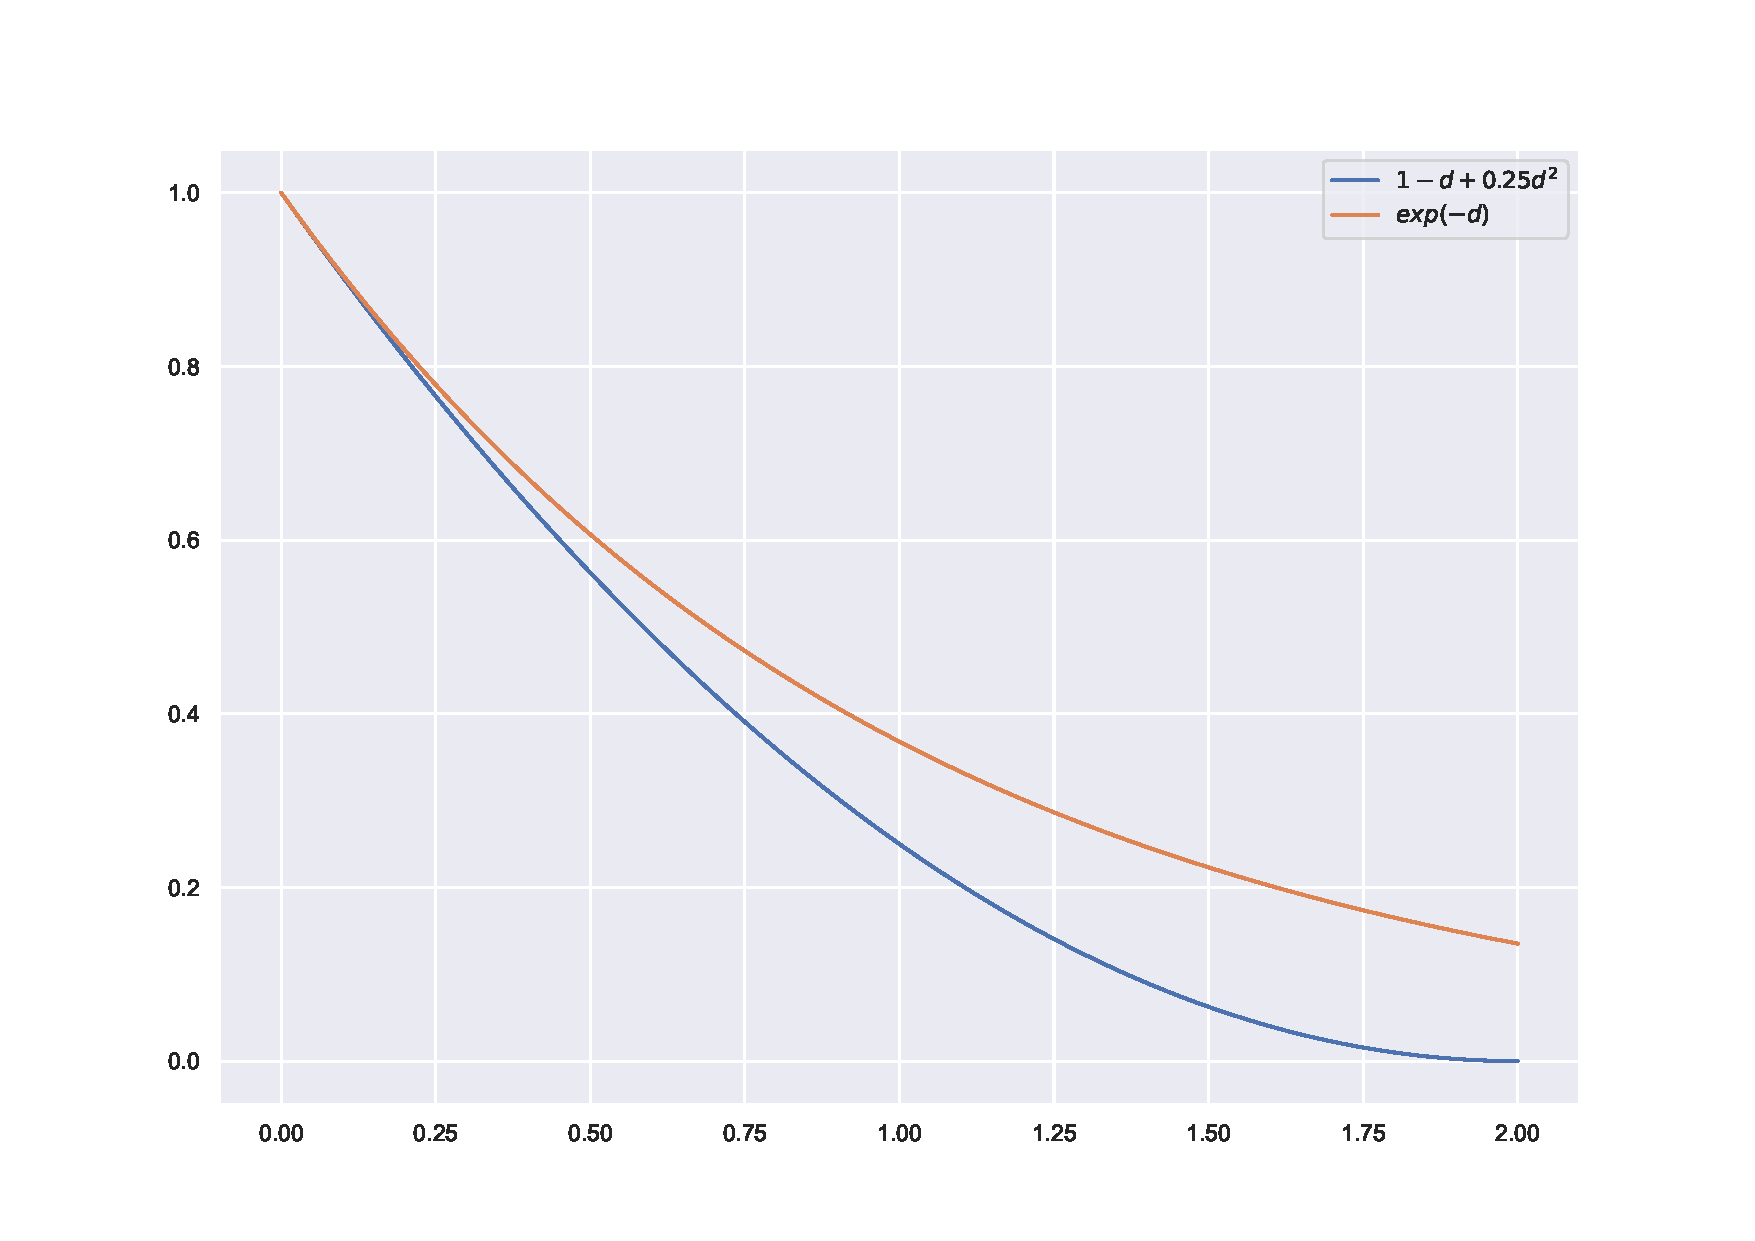
\includegraphics[width=\textwidth]{pics/hw6t4p1.pdf}
        \caption{Графики функций $\E\left[(X - d)^+\right]$ и $\E\left[(Y - d)^+\right]$ при $d\in[0, 2]$}
    \end{figure}
    Очевидно, что когда $d \geq 2$, то $0 = \E\left[(X - d)^+\right] < \E\left[(Y - d)^+\right]$. Таким образом, $X <_{sl} Y$.
    %\setcounter{ProblemNum}{0}\chapter{Порядок Лоренца. Операции, ослабляющие и сохраняющие порядок. Взвешивание и смеси.}
\problem{} 
Стохастический порядок не сохраняется для премии Эсшера. Пример: совместное распределение двух рисков $X$ и $Y$ задается следующим образом при некотором $h > 0$:
$P(X = 0, Y = 0) = 1/3$, $P(X = 0, Y = 2/(3h)) = 1/3,$
$P(X = 3/h, Y = 3/h) = 1/3$.\\
Необходимо проверить, что $X <_{st} Y$, но $\Pi_X > \Pi_Y $.

\solution{}
    Премия Эсшера:
    \begin{equation}
        \Pi(X, h) = \Pi_X = \frac{\E\left[Xe^{hX}\right]}{g_X(h)} =  \frac{g'_X(h)}{g_X(h)}
    \end{equation}
    Из условия следуют совместные распределения $X$ и $Y$:
    \begin{figure*}[htbp]\label{hw07:task1tab1}
        \begin{tabular}{|c|c|c|}\hline
            $x$ & $0$ & $3/h$ \\\hline
            $P(X = x)$ & $2/3$& $1/3$  \\\hline
        \end{tabular}
        \begin{tabular}{cccc}
            &&&
        \end{tabular}
        \begin{tabular}{|c|c|c|c|}\hline
            $y$ & $0$ & $2/(3h)$ & $3/h$ \\\hline
            $P(Y = y)$ & $1/3$ &$1/3$&$1/3$\\\hline
        \end{tabular}
    \end{figure*}

    По определению стохастического порядка получаем, что $X <_{st} Y$ (см. рис. \ref{hw07:task1pic1}).
    \begin{figure}[htbp]
        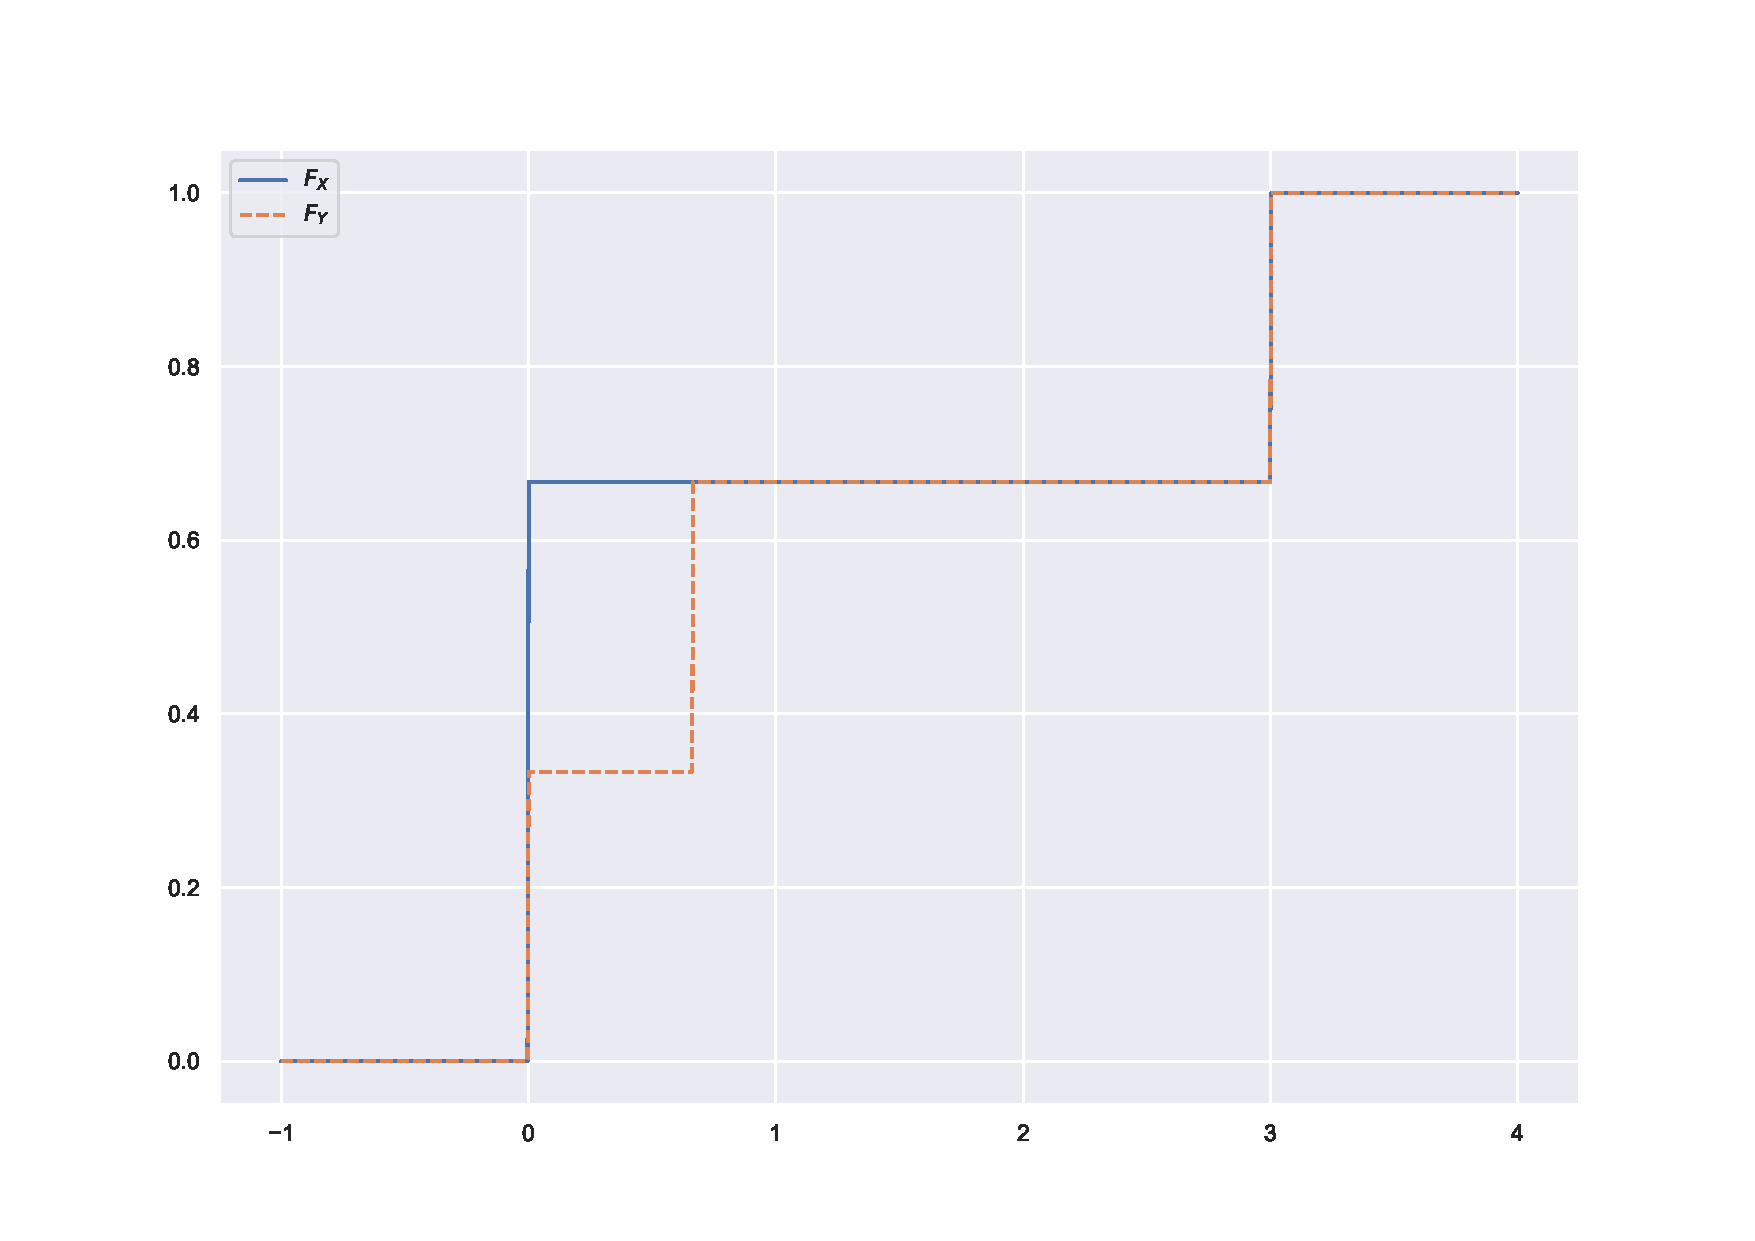
\includegraphics[width=\textwidth]{pics/hw7t1p1.pdf}\label{hw07:task1pic1}
        \caption{Функции распределения $X$ и $Y$}
    \end{figure}
    Теперь сравним соотвествующие премии:
    \begin{align}
        g_X(t) &= \frac{2}{3}+\frac{1}{3}e^{\frac{3}{h}t},  & g_X'(t) = \frac{1}{h}e^{\frac{3}{h}t};\\
        g_Y(t) &= \frac{1}{3}+\frac{1}{3}e^{\frac{3}{h}t} +\frac{1}{3}e^{\frac{2}{3h}t}, & g_Y'(t)=\frac{1}{h}e^{\frac{3}{h}t} +\frac{2}{9h}e^{\frac{2}{3h}t}.
    \end{align}
    Отсюда получаем
    \begin{align}
        \Pi_X &= \frac{\frac{1}{h}e^{3}}{\frac{2}{3}+\frac{1}{3}e^{\frac{3}{h}t}};\\
        \Pi_Y &= \frac{\frac{1}{h}e^{3} +\frac{2}{9h}e^{\frac{2}{3}}}{\frac{1}{3}+\frac{1}{3}e^{3} +\frac{1}{3}e^{\frac{2}{3}}}.
    \end{align}
    Посчитаем отношение премий:
    \begin{equation}
        \frac{\Pi_X}{\Pi_Y} \approx 1.02091201055381,
    \end{equation}
    что означает, что $\Pi_X > \Pi_Y$.


\problem{} Сохраняется ли стохастический порядок рисков при подсчете премий по принципу среднего квадратичного?

\solution{}
    Премия, посчитанная по принципу среднего квадратичного:
    \begin{equation}
        H(X) = \E\left[X\right] + \beta \std X.
    \end{equation}
    Пусть $X\sim Be(0.5)$, $Y\equiv 1$, $\beta = 2$. Тогда
    \begin{itemize}
        \item $\E\left[X\right] = 0.5$, $\std X = 0.5$, $H(X) = 1.5$;
        \item $\E\left[Y\right] = 1$, $\std Y = 0$, $H(Y) = 1$. 
    \end{itemize}
    Но $X<_{st}Y$. Значит, не сохраняется.

\problem{} Всегда ли принцип нулевой полезности обеспечивает премию с нагрузкой?

\solution{}
    Пусть экономический агент обладает склонностью к риску ($MU(x)$ не убывает). Тогда его функция полезности будет выпуклой. По неравенству Йенсена имеем
    \begin{equation}\label{hw07:task3eq1}
        \E\left[U(X)\right] \geq U\left(\E\left[X\right]\right).
    \end{equation}
    Премия, рассчитанная по принципу нулевой полезности, будет равна
    \begin{equation}\label{hw07:task3eq2}
        P\colon \quad \E\left[U(P-X)\right] = U(0).
    \end{equation}
    Из уравнений \eqref{hw07:task3eq1} и \eqref{hw07:task3eq2} следует, что
    \begin{equation}
        U(0) = \E\left[U(P-X)\right] \geq U\left(\E\left[P-X\right]\right) = U\left(P-\E\left[X\right]\right)
    \end{equation}
    Из монотонности полезности имеем, что 
    \begin{equation}
        0\geq P-\E\left[X\right] \implies P\leq\E\left[X\right]. 
    \end{equation}
    Поэтому эта премия не будет обеспечивать нагрузку.

\problem{} 
Как меняется в смысле порядка $<_e$ семейство показательных распределений при росте параметра?

\solution{}
    По определению: $X\leq_eY$, если $\forall \alpha > 0 \quad \E\left[e^{\alpha X}\right] \leq \E\left[e^{\alpha Y}\right]$.
    \begin{equation}
        \MGF(\alpha) = \begin{cases}
            \frac{\lambda}{\alpha-\lambda} & \alpha < \lambda, \\
            \infty & \alpha \geq \lambda.
        \end{cases}
    \end{equation}
    Очевидно, что по обоим аргументам функция строго монотонна на области определения. Поэтому экспоненциальный порядок сохраняет порядок на параметрах экспоненциального распределения.

\problem{} Экспоненциальный порядок не является полным порядком. Пример: $X$ имеет экспоненциальное распределение с
параметром $1$, а $Y$ - это смесь двух распределений, сосредоточенного в нуле и экспоненциального с параметром $1/2$, веса равны
соответственно $2/3$ и $1/3$. Проверить, что нельзя упорядочить указанные величины в смысле экспоненциального порядка.

\solution{}
    \begin{equation}
        \MGF_X(\alpha) = \begin{cases}
            \frac{1}{1-\alpha} & \alpha < 1, \\
            \infty & \alpha \geq 1.
        \end{cases}
    \end{equation}
    \begin{equation}
        \MGF_Y(\alpha) =\begin{cases}
            \frac{2}{3} + \frac{1}{3-6\alpha} & \alpha < \frac{1}{2}, \\
            \infty & \alpha \geq \frac{1}{2}.
        \end{cases}
    \end{equation}
    \begin{figure}[htbp]
        \begin{tabular}{|c|c|c|}\hline
              & $\MGF_X$ & $\MGF_Y$ \\\hline
            $\MGF$ & $\frac{1}{\alpha-1}$ & $\frac{2}{3} + \frac{1}{3- 6\alpha}$ \\\hline
            $\alpha = 1/6$ & $6/5$ & $7/6$ \\\hline
            $\alpha = 1/3$ & $3/2$ & $5/3$\\\hline
        \end{tabular}
    \end{figure}
    Отсюда видим, что распределения несравнимы в экспоненциальном смысле.
    \setcounter{ProblemNum}{0}\chapter{Виды и механизмы перестрахования. Пропорциональное перестрахование, квотный договор. Уравновешенность договора, экономические и финансовые условия}
\problem{}
Нарисовать кривую Лоренца для распределения Парето с $F(x) = 1 - (x/\sigma)^{-\alpha},$ $x \geq \sigma > 0$.
\solution{}

    Найдем квантильную функцию распределения $F$:
    \begin{equation*}
        y = 1 - (x/\sigma)^{-\alpha}  \; \Rightarrow \; x = \sigma(1 - y)^{-\frac{1}{\alpha}},
    \end{equation*}
    \begin{equation*}
        \int_0^u \sigma(1-t)^{-\frac{1}{\alpha}}dt = \int_{1-u}^1 \sigma s^{-\frac{1}{\alpha}}ds = \sigma \frac{\alpha - 1}{\alpha}\left(1 - (1 - u)^{\frac{\alpha - 1 }{\alpha}}\right).
    \end{equation*}
    Следовательно 
    \begin{equation*}
        L_X(u) = 1 - (1 - u)^{\frac{\alpha- 1}{\alpha}}.
    \end{equation*}
    См Рис \ref{fig:hw8t1p1}.

    \begin{figure}[htbp]
        \centering
        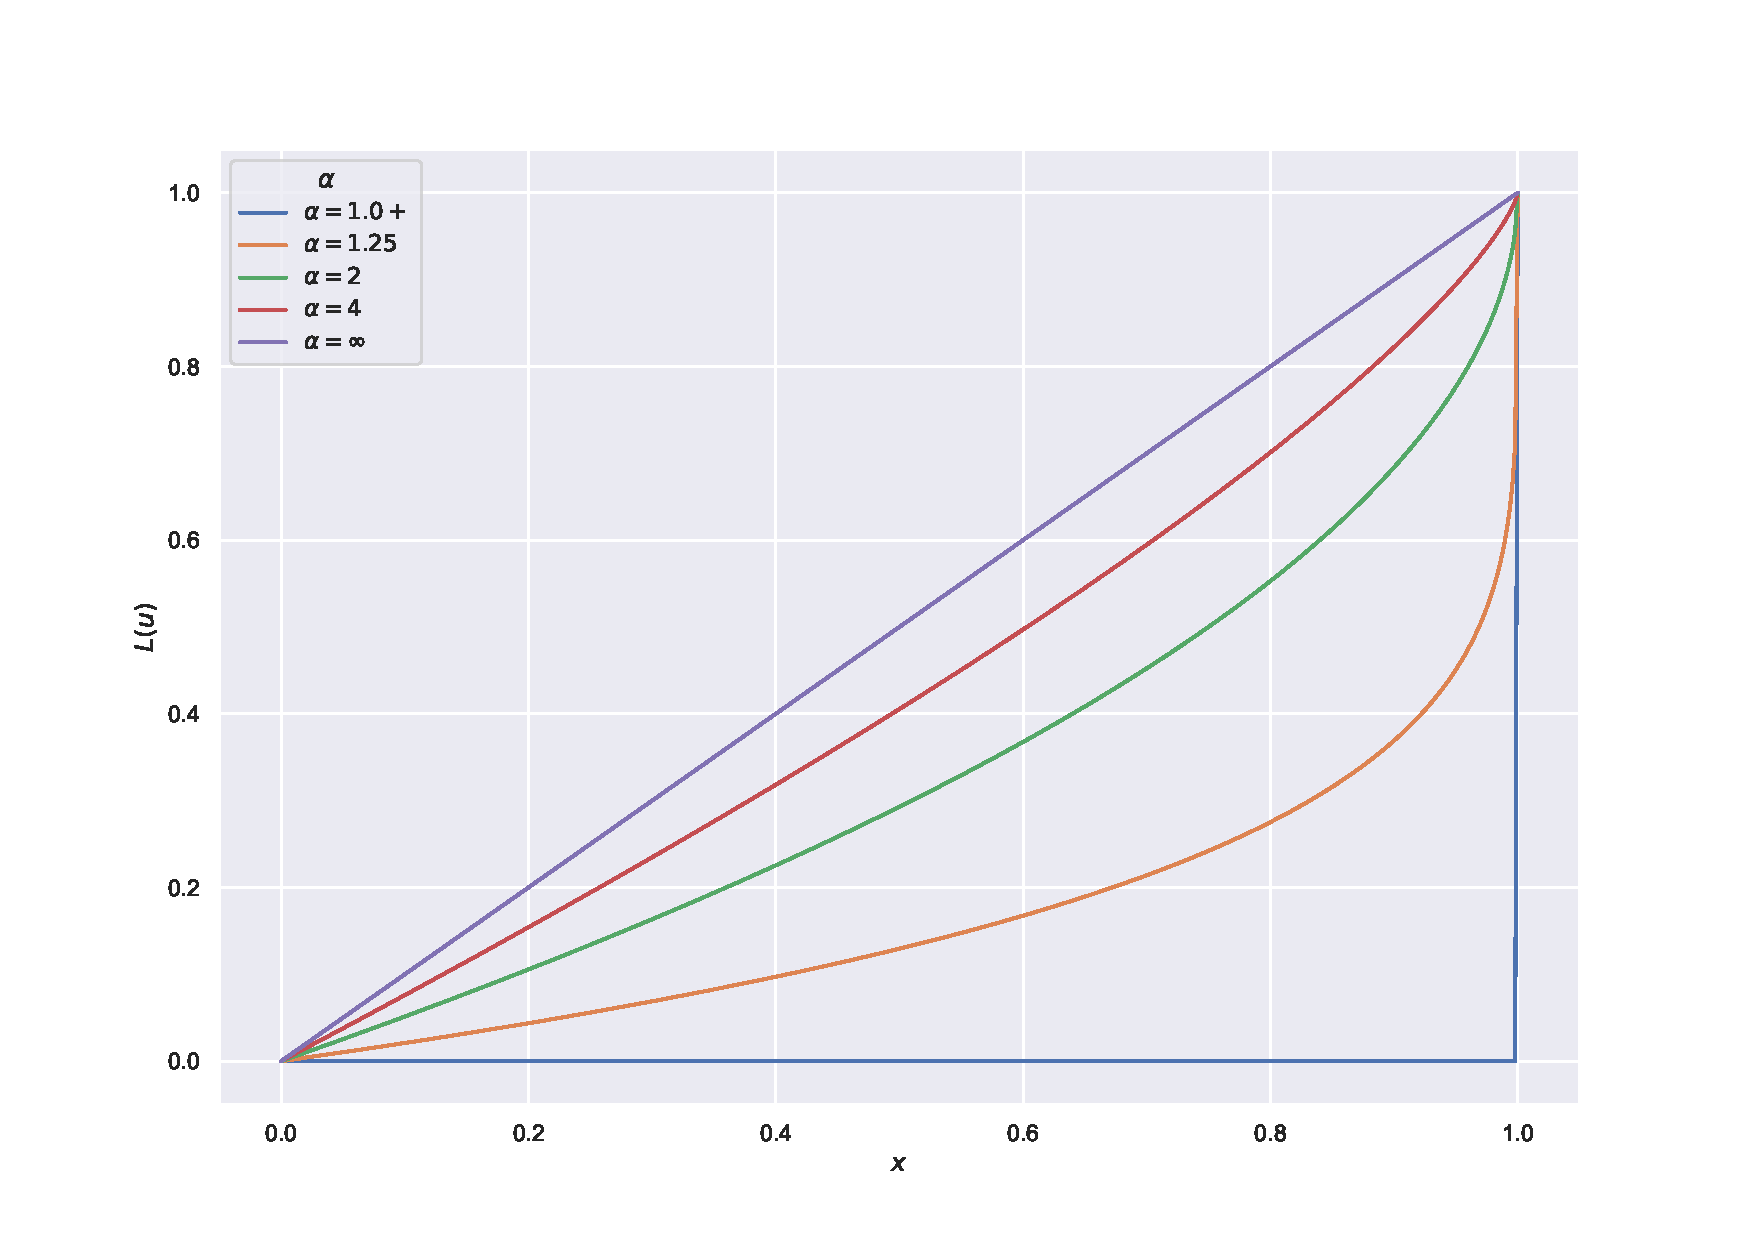
\includegraphics[width=\linewidth]{pics/hw8t1p1.pdf}
        \caption{Кривая Лоренца для распределения Парето с разными параметрами}
        \label{fig:hw8t1p1}
    \end{figure}

\problem{}
Проверить, что если $X \prec_{Lor} Y$, то $CV(X) \leq CV(Y)$. Верно ли обратное утверждение?
\solution{}

$$X \prec_{Lor} Y \iffdef \frac{X}{\E[X]} <_{cx} \frac{Y}{\E[Y]}$$
Имеем: 
\begin{align}
    & \E [X^2] / (\E [X])^2 \leq \E[Y^2 ]/ (\E[Y])^2, \\
    & (\E[X^2] - (\E[X])^2)/ (\E[X])^2 \leq (\E[Y^2] - (\E[Y])^2) / (\E[Y])^2.
\end{align}
Взяв квадратный корень от обех частей получаем требуемое утверждение.
Чтобы показать, что обратное неверно, возьмем случайные величины $X,Y$ со средним, равным $1$, $X<C=const$ п.н., $Y$ - неограничена, и $\var X > \var Y $. Подойдут например $X: \P(X=0) = 2/3, \P (X = 3) = 1/3$ и $Y \sim Exp(1).$ Тогда $\sqrt 2 = CV(X) > CV(Y) = 1 $. Но $\E(X - 3)^+ = 0 < \E(Y - 3)^+ = e^{-3}$. Значит, либо $X<_{cx} Y$ либо $X$ и $Y$ - несравнимы. 

\problem{}
Пусть $X$ и $Z$ - независимые случайные величины, $X \sim \Gamma(1, \lambda^{-1})$, $Z \sim \Gamma(\alpha, 1)$. Проверить, что $Y = X/Z$ имеет распределение Парето с функцией распределения $F(x) = 1 - (x/\sigma)^{-\alpha},$ $x \geq \sigma > 0$.
\solution{}

\begin{multline*}
    \iint_{x/y \leq t} f_{X,Y}(x,y)dxdy = \iint_{x/y \leq t} f_{X}(x) f_Y(y)dxdy =\\= \left[x/y = u, x = v \right] =
    \int_{u\leq t}\int_{v \in \mathbb R}f_X(v)f_Y(v/u)\frac{|v|}{u^2}dvdu =\\= 
    \int_{0\leq u\leq t}\int_0^{+\infty} \frac{1}{\lambda}e^{v/\lambda} \frac{1}{\Gamma(\alpha)}\left( \frac{v}{u}\right)^{\alpha - 1} e^{-v/u} \frac{v}{u^2} dv du =\\= 
    \int_{0\leq u\leq t}\frac{1}{\Gamma(\alpha) u^{\alpha +1} \lambda}\int_0^{+\infty} v^\alpha \exp\left(-(\frac1\lambda + \frac1u)v\right) dv du =\\= 
    \int_{0\leq u\leq t}\frac{(\frac1\lambda + \frac1u)^{-(\alpha +1)}}{\Gamma(\alpha) u^{\alpha +1} \lambda}\int_0^{+\infty} s^\alpha \exp\left(-s\right) ds du =\\= \frac{\Gamma(\alpha + 1)}{\lambda\Gamma(\alpha)} \int_{0\leq u\leq t} \left(\frac u\lambda + 1 \right)^{-\alpha - 1}du = \alpha \int_1^{1+ t/\lambda} s^{-\alpha - 1}ds = \\ = 1 - (1 + t/\lambda)^{-\alpha}.
\end{multline*}

\problem{}
Показать, что $ X <_{st} Y \not\Rightarrow X <_k Y $. (Указание: рассмотреть $X \sim U(0, 2)$, $Y \sim U(1, 2)$, где $U(a, b)$ - равномерное
распределение на $(a, b)$.)
\solution{}
Рассмотрим предложенные случайные величины. $X^* = X/\mathbb E[X] = X, Y^* = Y/\mathbb E [Y] = \frac{2}{3}Y$. Для любого $t$ $F_X(t)\geq F_Y(t) \iff X<_{st} Y$. Однако, $\frac{2}{3}Y \sim U(2/3, 4/3)$ и $\mathbb E[(X^* - 4/3)^+] = 1/3 > \mathbb E [(Y^* - 4/3)^+] = 0$. Следовательно, $X^*$ и $Y^*$ либо несравнимы, либо $Y^* <_{sl} X^*$. Осталось вспомнить, что $Y^* <_{sl} X^* \Leftrightarrow Y <_{k} X_{k}$.

\problem{}
Показать, что $X <_k Y \not\Rightarrow X <_{st} Y$. (Указание: рассмотреть $X \sim Exp(1)$, $Y \sim Exp(2)$, где $Exp(a)$ - показательное
распределение с параметром $a$.)
\solution{}
Рассмотрим предложенные случайные величины. $X^* = X/\mathbb EX = X, \; Y^* = Y/\mathbb E Y = 2 Y \sim X \Rightarrow X^*<_{sl} Y^*$, но $\bar F_Y(x) = e^{-2x} < e^{-x} = \bar F_X(x), \; x\geq 0 \Rightarrow Y<_{st}X$.

\problem{}
Проверить, что гамма-распределение с $\alpha \geq 1$ и равномерное имеют тип IFR.
\solution{}
\begin{enumerate}
    \item Случай гамма распределения. Для простоты будем рассматривать $1/\lambda(x)$. Необходимо показать, что $1/\lambda(x) $ - убывает по $x$. 
    \begin{equation*}
        1/\lambda(x) = \left( \frac{\beta^\alpha x^{\alpha - 1}}{\Gamma(\alpha)} \right)^{-1} \int_x^\infty \frac{\beta^\alpha t^{\alpha - 1}}{\Gamma(\alpha)}e^{-\beta t} dt = \left[ t - x = u, dt = du \right] = \int_0^\infty \left(\frac{u}{x} + 1\right)^{\alpha -1}e^{-\beta u} du
        \end{equation*}
        не возрастает по $x$ при $\alpha \geq 1$.

    \item Случай равномерного распределения $U(a,b)$.
    \begin{equation*}
        \lambda(x) =\frac{\frac{1}{b-a}}{1 - \frac{x - a}{b - a}} =  \frac{1}{b - x},
    \end{equation*}
    Это выражение возрастает по $x$.
\end{enumerate}

\problem{}
Показать, что если $X_i <_{mor} Y_i$, $i \geq 1$, то $\min_i X_i <_{mor} \min_i Y_i$.
\solution{}

Напомним, что $F_{\min_i X_i} (x) = 1 - (1 - F(x))^n$. Действительно, $\P( \min_i X_i < x) $ означает, что хотя бы 1 из $X_i$ меньше либо равен $x$. Это тоже самое, что
    \begin{equation*}
        \sum_{k =1}^n \mathbb{P}(X_{(k)} \leq x, X_{(k+1)} > x ) =  \sum_{k=1}^n \binom{n}{k} F^k(x)(1 - F(x))^{n-k} = 1 - (1 - F(x))^n.
    \end{equation*}
    Отсюда, поскольку $\frac{1 - F_X(x)}{1 - F_Y(x)}$ убывает по $x$, то 
    \begin{equation*}
        \frac{1 - F_{\min_i X_i}(x)}{ 1 - F_{\min_i Y_i}(x)} = \left( \frac{1 - F_X(x)}{ 1 - F_Y(x)} \right)^n
    \end{equation*}
    убывает по $x$ и, следовательно, $\min_i X_i <_{mor} \min_i Y_i$.
    \setcounter{ProblemNum}{0}\chapter{Непропорциональное страхование. Экцедент убытка по риску/катастрофе. Финансовые и экономические условия.}
\problem{}
Рассматривается договор эксцедента убытка по риску $XL$: $5\, xs\, 2$. Предполагается, что возможны 4 возобновления. Добавочные премии за возобновление полосы: $25\%$, $50\%$, $100\%$, $200\%$.  Произошло $8$ убытков, их размеры: $5$, $10$, $7$, $4$, $6$, $8$, $3$, $9$. Первоначальная премия равна 4. 
Подсчитать размер добавочных премий. Все размеры в млн. 

\solution{}
Пусть $X_i$ -- указанные убытки, $Y:= \min\left\{5, (X_i-2)_+\right\}$ -- перестраховое покрытие, $L = 5\cdot\left(4+1\right) = 25 $ -- максимальное значение гарантий перестраховщика, $Y = \sum_{i=1}^8 Y_i$ -- суммарные выплаты по обязательствам перестраховщика.
\begin{table}[h]\centering
    \begin{tabular}{|c|c|c|c|c|c|}\hline
        $i$ & $X_i$ & $Y_i$ & $Y$ & $XL$ & добавочная премия \\\hline\hline
        1   & 3     & 3     &  3   &  3   & 0.6 \\\hline
        2   & 10    & 5     &  8   &  5   & 1.6 \\\hline
        3   & 7     & 5     &  13  &  5   & 3.2 \\\hline
        4   & 4     & 2     &  15  &  2   & 1.6 \\\hline
        5   & 6     & 4     &  19  &  4   & 6.4 \\\hline
        6   & 8     & 5     &  24  &  5   & 1.6 \\\hline
        7   & 3     & 1     &  25  &  1   & --- \\\hline
        8   & 9     & 5     &  30  & ---  & --- \\\hline
    \end{tabular}
\end{table}

Добавочные премии закончились на $7$-м убытке, т.к. мы достигли максимальных гарантий перестраховщика.






\problem{}

Подсчитать, чему равна премия по договору $3 \,xs\, 2$ (млн.), если размеры последовательных убытков равнялись $3$, $3.4$, $3.2$, $4.8$, $4.4$, $7$. 
Предполагается, что применяется скользящая ставка премии от $2\%$ до $5\%$ (при коэффициенте надбавки $100/80$ убытков на гарантии 
перестраховщика, уже оплаченных или еще не урегулированных). Премия прямого страховщика равна $200\cdot 10^6$. 

\solution{}
Пусть $X_i$ -- указанные убытки, $Y:= \min\left\{3, (X_i-2)_+\right\}$ -- перестраховое покрытие, $Y = \sum_{i=1}^6 Y_i = 11.8$.
\begin{equation}
    r = \min\{\underbrace{r_{\max}}_{5\%}, \underbrace{\max\{\underbrace{r_{\min}}_{2\%}, \underbrace{\tfrac{dY}{A}}_{=\frac{100\times 11.8}{8\times 200} = 73.75\%}\}}_{73.75\%}\} = 5\%.
\end{equation}
Итого, $P = rA = .05\times 200 = 10$.
    \setcounter{ProblemNum}{0}\chapter{Оптимальное перестрахование. Порядки рационального перестраховщика, эксцедента богатства и рассеивания.}
\problem{}

\solution{}
\begin{itemize}
    \item Пусть $X \sim U[0,2b]$. Тогда
    \begin{multline}
        \pi_\rho(X) = \int_0^{2b} (1 - t/(2b) ) ^{\frac{1}{\rho}} dt =\\= [ 1 - t/(2b) = y,  -2bdy = dt] = 2b\int_0^1 y^{\frac1\rho} dy = 2b \frac{1}{\frac{1}{\rho} + 1} = \frac{2b\rho}{1 + \rho}.
    \end{multline}
    Подставляя значения $\rho$ получаем $\pi_{1.2}(X) = \frac{2.4 b}{2.2} = 1.1b$, $\pi_{1.5}(X) = \frac{3 b}{2.5} = 1.2b$, $\pi_{1.8}(X) = \frac{3.6 b}{2.8}= 1.29b$
    \item Пусть $Y \sim \exp(1/b)$. Тогда 
    \begin{equation}
        \pi_\rho(Y) = \int_0^{+\infty} \exp(-t/(b\rho)) dt = b\rho .
    \end{equation}
     Подставляя значения $\rho$ получаем  $\pi_{1.2}(Y) = 1.2b$, $\pi_{1.5}(Y) = 1.5b$,  $\pi_{1.8}(Y) = 1.8b$.

     \item Пусть $Z \sim \bar F_Z(t) = b^2 /(b+t)^2$. Тогда 
     \begin{multline}
         \pi_\rho(Y) = \int_0^{+\infty} b^{2\rho}/(b+ t)^{2\rho} dt =\\= [ y = b + t, dy = dt] = b^{2\rho}\int\limits_{b}^{+\infty} y^{-2\rho}dy = \frac{b}{2\rho - 1},  \rho>1/2.
     \end{multline}
     Подставляя  значения $\rho$ получаем $\pi_{1,2}(Z) = b/1.4$, $\pi_{1,5}(Z) = b/2$, $\pi_{1,8}(Z) = b/2.6$.
\end{itemize}
    \setcounter{ProblemNum}{0}\chapter{Апостериорная тарификация. Теория ограниченных флуктуаций. Модель Бюлмана.}

    \problem{}
    Найти наилучшее приближение $X_{t+1}$ c помощью неоднородной линейной комбинации $X_1,\dots, X_t$. 
    
    \solution{}
        Ищем оценку в следующем виде:
        \begin{align}
            & \hat X_{t+1} = \beta \cdot \mathbb{X}_t, \quad \mathbb{X}_t = \left[1, X_1, X_2, \dots, X_t\right]^T, \quad \beta = [\beta_0, \dots, \beta_t], \\
            & \forall s = 0, \dots, t \quad \cov\left[X_{t+1} - \hat X_{t+1}, X_s\right] = 0
        \end{align}
        Очевидно, что из $X_0 = 1$ следует несмещенность оценки и выражение $\beta_0$ через другие коэффициенты:
        \begin{equation}
            \beta_0 = \left(1 - \sum_{s = 1}^t \beta_s\right)m.
        \end{equation}
        В частности, \begin{equation}
            0 = \cov\left[X_{t+1} - \hat X_{t+1}, X_s\right] = \E\left[\left(X_{t+1} - \hat X_{t+1}\right) X_s\right].
        \end{equation}
        Итого, 
        \begin{multline}
            \cov\left[X_{t+1} - \hat X_{t+1}, X_s\right] = \cov\left[X_{t+1}, X_s\right] - \sum_{u = 0}^t\beta_u\cov\left[X_{u}, X_s\right] =\\=
            a - \sum_{u = 1, u \neq s}^t\beta_ua - \beta_s(a+s^2) = 0,
        \end{multline}
        откуда имеем
        \begin{equation}
            \forall i = 1, \dots, t\quad  \beta_is^2 = a\left(1 - \sum_{s = 1}^t \beta_s\right) \implies \forall i = 1, \dots, t\quad  \beta_i = \frac{a}{at + s^2}.
        \end{equation}

    \problem{}
    Найти наилучшее приближение $\mu(\Theta)$ c помощью однородной линейной комбинации $X_1,\dots,X_t$. 
    
    \solution{}
        Ищем оценку в следующем виде:
        \begin{align}
            & \hat \mu = \beta \cdot \mathbb{X}_t, \quad \mathbb{X}_t = \left[X_1, X_2, \dots, X_t\right]^T, \quad \beta = [\beta_1, \dots, \beta_t], \\
            & \forall s = 0, \dots, t \quad \cov\left[X_{t+1} - \hat X_{t+1}, X_s\right] = 0.
        \end{align}
        \begin{multline}
            \E\left[\left(\mu(\theta) -\hat \mu\right)X_s\right] = \cov\left[\mu(\theta) -\hat \mu, X_s\right] = 
            \cov\left[\mu(\theta), X_s\right] - \cov\left[\hat \mu, X_s\right] = \\=
            \cov\left[\mu(\theta), X_s\right] - \sum_{u = 1}^t\beta_u\cov\left[X_u, X_s\right] + \E[X_s]\left(\E\left[\mu(\theta)\right] - \sum_{u=1}^{t}\beta_u\E\left[X_u\right]\right) = \\ =
            a - \sum_{u=1}^{t}\beta_ua - \beta_ss^2 +m^2\left(1 - \sum_{u=1}^{t}\beta_u\right) =0
        \end{multline}
        Итого,
        \begin{equation}
            \beta_{...} = \frac{a+m^2}{(a+m^2)t + s^2} 
        \end{equation}

    \problem{}
    Проверить, пользуясь тем, что $X_{t+1}$ и  $X_1,\dots,X_t$ условно независимы при данной $\Theta$,   равенство 
    $$ E(X_{t+1}|X_1,\dots,X_t)=E(\mu(\Theta)|X_1,\dots,X_t).$$ 
    
    \solution{}
        $\mu(\Theta) := \E\left[X_i\vert \Theta\right]$. Знаем, что
        \begin{equation}
            \E\left[X_{t+1} \vert X_1, \dots, X_t, \Theta\right] = \E\left[X_{t+1} \vert \Theta\right] = \mu(\Theta).
        \end{equation}
        Имеем
        \begin{multline}
            \E\left[\mu(\Theta)\vert X_1,\dots, X_t\right] = \E\left[ \E\left[X_{t+1} \vert \Theta\right]\vert X_1,\dots, X_t\right] = \\= 
            \E\left[ \E\left[X_{t+1} \vert X_1, \dots, X_t, \Theta\right] \vert X_1,\dots, X_t\right] \overset{\text{iterated expectations}}{=}  \E\left[X_{t+1}  \vert X_1,\dots, X_t\right]
        \end{multline}


\end{document}


